\باب{مخروطی حصے، منحنی مقدار معلوم اور قطبی محدد}

\جزوحصہء{جائزہ}
حرکت پر غور احصاء کی مدد سے کیا جا سکتا ہے۔ اس حصہ میں ہم وقت کے ساتھ ایک ذرے کے بدلتے مقام پر غور کریں گے۔ ہم  مخروطی حصوں کی مساوات سے شروع کرتے ہیں چونکہ بالعکس مربع قوت کی بنا سیارے، مصنوعی سیارے، اور دیگر اجسام  مخروطی راہ پر حرکت کرتے ہیں۔ اگر ہمیں معلوم ہو کہ ایک جسم مخروطی راہ پر حرکت کر رہا ہے  تب ہم اس کی رفتار اور اس پر عمل کرنے والی قوت دریافت کر سکتے ہیں۔  قطبی محدد سیاروں کی حرکت پر غور کو بہت آسان بناتا ہے لہٰذا ہم اس نئے محدد میں منحنیات، تفرق اور تکمل پر بھی غور کریں گے۔

\حصہ{مخروطی حصے اور دو قدری مساواتیں}
اس حصہ میں دکھایا جائے گا کہ مخروطی حصوں کو کس  طرح محددی سطح پر بطور دو قدری مساوات پیش کیا جاتا ہے۔ دوہرے مخروط کو سطح سے کاٹ کر مخروطی منحنیات پیدا کی جاتی ہیں اور اسی کی بنا مخروطی حصہ کی اصطلاح پیدا ہوئی۔

\جزوحصہء{دائرہ}
\ابتدا{تعریف}
ایک مستوی میں رہتے ہوئے اس مستوی میں کسی مقررہ نقطہ سے مستقل فاصلے پر تمام نقطوں کے سلسلہ کو \اصطلاح{دائرہ}\فرہنگ{دائرہ}\حاشیہب{circle}\فرہنگ{circle} کہتے ہیں۔ اس مقررہ نقطہ کو دائرے کا \اصطلاح{مرکز}\فرہنگ{مرکز}\حاشیہب{center}\فرہنگ{center} کہتے ہیں جبکہ اس مستقل فاصلہ کو \اصطلاح{رداس}\فرہنگ{رداس}\حاشیہب{radius}\فرہنگ{radius} کہتے ہیں۔ 
\انتہا{تعریف}
 
 دائرے کے معیاری مساوات جنہیں حصہ \حوالہ{حصہ_ابتدا_ترسیم_کی_منتقلی} میں فاصلہ کی مساوات \عددی{d=\sqrt{(x_2-x_1)^2+(y_2-y_1)^2}} سے اخذ کیا گیا درج ذیل ہیں۔
\begin{align*}
x^2+y^2&=a^2&&\text{\RL{رداس \عددی{a} اور مرکز \عددی{(0,0)}}}\\
(x-h)^2+(y-k)^2&=a^2&&\text{\RL{رداس \عددی{a} اور مرکز \عددی{(h,k)}}}
\end{align*}

\جزوحصہء{قطع مکافی}
\ابتدا{تعریف}
ایک سطح میں رہتے ہوئے کسی مقررہ سیدھی لکیر اور مقررہ نقطہ (جو اس مقررہ سیدھی لکیر پر نہیں پایا جاتا ہو) سے مستقل فاصلہ پر پائے جانے والے تمام نقطوں کے سلسلہ کو \اصطلاح{قطع مکافی}\فرہنگ{قطع مکافی}\حاشیہب{parabola}\فرہنگ{parabola} کہتے ہیں۔مقررہ نقطے کو قطع مکافی کا \عددی{ماسکہ}\فرہنگ{ماسکہ}\حاشیہب{focus}\فرہنگ{focus} کہتے ہیں جبکہ مقررہ لکیر کو \اصطلاح{ناظمہ}\فرہنگ{ناظمہ}\حاشیہب{directrix}\فرہنگ{directrix} کہتے ہیں۔ 
\انتہا{تعریف}
%==============

جب ماسکہ کسی محددی محور پر ہو اور ناظمہ اس محددی محور کے متوازی ہو تب قطع مکافی کی مساوات سادہ ترین ہوتی ہے۔مثال کے طور پر، فرض کریں کہ ماسکہ \عددی{y} محور پر نقطہ \عددی{F(0,p)} پر پایا جاتا ہے اور لکیر \عددی{y=-p} ناظمہ (شکل \حوالہ{شکل_مخروط_قطع_مکافی_الف})  ہے۔ یوں شکل \حوالہ{شکل_مخروط_قطع_مکافی_الف} میں نقطہ \عددی{N(x,y)} صرف اور صرف اس صورت اس قطع مکافی پر پایا جائے گا جب \عددی{NF=NQ} ہو۔ فاصلہ کے کلیہ سے
\begin{align*}
NF&=\sqrt{(x-0)^2+(y-p)^2}=\sqrt{x^2+(y-p)^2}\\
NQ&=\sqrt{(x-x)^2+(y-(-p))^2}=\sqrt{(y+p)^2}
\end{align*}
لکھا جا سکتا ہے۔ ان مساوات کو ایک دوسرے کے برابر پر کر کے حل کرتے ہوئے درج ذیل حاصل ہو گا۔
\begin{align}\label{مساوات_مخروط_قطع_مکافی_معیاری_الف}
y&=\frac{x^2}{4p}\quad \implies \quad x^2=4py&&\text{\RL{معیاری روپ}}
\end{align}
اس مساوات سے قطع مکافی کی \عددی{y} محور کے لحاظ سے تشاکلی واضح ہے۔ ہم کہتے ہیں کہ محور \عددی{y} اس قطع مکافی کا محور تشاکلی ہے جس کو عموماً چھوٹا کر کے صرف \اصطلاح{محور}\فرہنگ{محور}\حاشیہب{axis}\فرہنگ{axis} پکارا جاتا ہے۔

وہ نقطہ جس پر قطع مکافی اپنے محور کو قطع کرتا ہو \اصطلاح{راس}\فرہنگ{راس}\حاشیہب{vertex}\فرہنگ{vertex} کہلاتا ہے۔ قطع مکافی \عددی{x^2=4py} کا راس مبدا پر پایا جاتا ہے (شکل \حوالہ{شکل_مخروط_قطع_مکافی_الف})۔ مثبت عدد \عددی{p} کو قطع مکافی کا \اصطلاح{طول ماسکہ}\فرہنگ{ماسکہ!طول}\حاشیہب{focal length}\فرہنگ{focal!length} کہتے ہیں۔
\begin{figure}
\centering
\begin{minipage}{0.45\textwidth}
\centering
\begin{tikzpicture}[declare function={f(\x)=1/4*\x^2;}]
\pgfmathsetmacro{\a}{1.5}
\pgfmathsetmacro{\b}{f(\a)}
\begin{axis}[clip=false,small,axis lines=middle, xtick={\empty},ytick={\empty}, enlargelimits=true,ymin=-1.25, xlabel={$x$},ylabel={$y$}, xlabel style={at={(current axis.right of origin)},anchor=west},ylabel style={at={(current axis.above origin)},anchor=south}]
\addplot[domain=-2.5:2.5]{f(x)}node[pos=0.1,left]{$x^2=4py$};
\addplot[]plot coordinates {(0,1)}node[circ]{}node[left]{ماسکہ}node[above right]{$F(0,p)$};
\addplot[]plot coordinates {(0,1)(\a,\b)}node[circ]{}node[right]{$N(x,y)$};
\addplot[]plot coordinates {(-2.5,-1)(2.5,-1)}node[right]{$L$}node[pos=0.25,above]{ناظمہ}node[pos=0.25,yshift={-0.5ex},below]{$y=-p$};
\addplot[dashed] plot coordinates {(\a,\b)(\a,-1)}node[circ]{}node[below]{$Q(x,-p)$};
\addplot[]plot coordinates {(0,0.5)}node[left]{$p$};
\addplot[]plot coordinates {(0,-0.5)}node[left]{$p$};
\addplot[]plot coordinates {(0,0)}node[circ]{}node[below right]{راس};
\end{axis}
\end{tikzpicture}
\caption{قطع مکافی \عددی{x^2=4py}؛ راس کا فاصل ماسکہ اور ناظمہ سے ایک جیسا ہے۔}
\label{شکل_مخروط_قطع_مکافی_الف}
\end{minipage}\hfill
\begin{minipage}{0.45\textwidth}
\centering
\begin{tikzpicture}[declare function={f(\x)=-1/4*\x^2;}]
\pgfmathsetmacro{\a}{1.5}
\pgfmathsetmacro{\b}{f(\a)}
\begin{axis}[clip=false,small,axis lines=middle,xtick={\empty},ytick={\empty},enlargelimits=true,ymin=-1.25,xlabel={$x$},ylabel={$y$},xlabel style={at={(current axis.right of origin)},anchor=west},ylabel style={at={(current axis.above origin)},anchor=south}]
\addplot[domain=-2.5:2.5]{f(x)}node[pos=0.2,left]{$x^2=-4py$};
\addplot[]plot coordinates {(0,-1)}node[circ]{}node[left]{ماسکہ}node[right]{$F(0,-p)$};
\addplot[]plot coordinates {(-2.5,1)(2.5,1)}node[right]{$L$}node[pos=0.25,above]{ناظمہ}node[pos=0.25,yshift={-0.5ex},below]{$y=p$};
\addplot[]plot coordinates {(0,0)}node[circ]{}node[above left]{\RL{راس مبدا پر ہے}};
\end{axis}
\end{tikzpicture}
\caption{قطع مکافی \عددی{x^2=-4py}}
\label{شکل_مخروط_قطع_مکافی_ب}
\end{minipage}
\end{figure}

اگر قطع مکافی نیچے رخ کھلتا ہو اور اس کا ماسکہ \عددی{(0,-p)} جبکہ ناظمہ لکیر \عددی{y=p} ہو تب مساوات \حوالہ{مساوات_مخروط_قطع_مکافی_معیاری_الف} درج ذیل روپ اختیار کرے گی (شکل \حوالہ{شکل_مخروط_قطع_مکافی_ب})۔
\begin{align*}
y=-\frac{x^2}{4p}\quad \implies \quad x^2=-4py
\end{align*}
ہم اسی طرح کے مساوات ہم دائیں اور بائیں کھلنے والے قطع مکافی کے لئے حاصل کر سکتے ہیں (جدول \حوالہ{جدول_مخروط_کھلنے_کی_سمت} اور شکل \حوالہ{شکل_مخروط_قطع+مکافی_بائیں_دائیں})۔

\begin{table}
\caption{مبدا پر راس والے قطع مکافی کے معیاری مساوات (\عددی{p>0})}
\label{جدول_مخروط_کھلنے_کی_سمت}
\centering
\begin{tabular}{LCLCC}
\text{مساوات}&\text{ماسکہ}&\text{ناظمہ}&\text{محور}&\text{\RL{کھلنے کا رخ}}\\
\toprule
x^2=4py&(0,p)&y=-p&\text{\عددی{y} محور}&\text{اوپر}\\
x^2=-4py&(0,-p)&y=p&\text{\عددی{y} محور}&\text{نیچے}\\
y^2=4px&(p,0)&x=-p&\text{\عددی{x} محور}&\text{دائیں}\\
y^2=-4px&(-p,0)&x=p&\text{\عددی{x} محور}&\text{بائیں}
\end{tabular}
\end{table}

\begin{figure}
\centering
\begin{subfigure}{0.45\textwidth}
\centering
\begin{tikzpicture}[declare function={fp(\x)=sqrt(4*\x);fn(\x)=-sqrt(4*\x);}]
\begin{axis}[clip=false,small,axis lines=middle,xlabel={$x$},ylabel={$y$},xtick={\empty},ytick={\empty},xlabel style={at={(current axis.right of origin)},anchor=west},ylabel style={at={(current axis.above origin)},anchor=south},xmin=-1.25]
\addplot[domain=0:0.2]{fp(x)};
\addplot[domain=0:0.2]{fn(x)};
\addplot[domain=0.2:2]{fp(x)}node[pos=0.75,above left]{$y^2=4px$};
\addplot[domain=0.2:2]{fn(x)};
\addplot[]plot coordinates {(1,0)}node[circ]{}node[above]{ماسکہ}node[below]{$F(p,0)$};
\addplot[]plot coordinates {(0,0)}node[circ]{}node[above left]{راس};
\addplot[]plot coordinates {(-1,-3)(-1,3)}node[pos=0.8,left]{ناظمہ}node[pos=0.8,below]{\scriptsize{$x=-p$}};
\end{axis}
\end{tikzpicture}
\end{subfigure}\hfill
\begin{subfigure}{0.45\textwidth}
\centering
\begin{tikzpicture}[declare function={fp(\x)=sqrt(4*\x);fn(\x)=-sqrt(4*\x);}]
\begin{axis}[clip=false,small,axis lines=middle,xlabel={$x$},ylabel={$y$},xtick={\empty},ytick={\empty},xlabel style={at={(current axis.right of origin)},anchor=west},ylabel style={at={(current axis.above origin)},anchor=south},xmax=1.25]
\addplot[domain=0:0.2]({-x},{fp(x)});
\addplot[domain=0:0.2]({-x},{fn(x)});
\addplot[domain=0.2:2]({-x},{fp(x)})node[pos=0.75,above right]{$y^2=-4px$};
\addplot[domain=0.2:2]({-x},{fn(x)});
\addplot[]plot coordinates {(-1,0)}node[circ]{}node[above]{ماسکہ}node[below]{$F(-p,0)$};
\addplot[]plot coordinates {(0,0)}node[circ]{}node[above right]{راس};
\addplot[]plot coordinates {(1,-3)(1,3)}node[pos=0.8,right]{ناظمہ}node[pos=0.8,below right]{\scriptsize{$x=p$}};
\end{axis}
\end{tikzpicture}
\end{subfigure}
\caption{قطع مکافی \عددی{y^2=4px} اور \عددی{y^2=-4px} کے ترسیمات۔}
\label{شکل_مخروط_قطع+مکافی_بائیں_دائیں}
\end{figure}

\ابتدا{مثال}
قطع مکافی \عددی{y^2=10x} کا ماسکہ اور ناظمہ تلاش کریں۔

حل:\quad
ہم معیاری مساوات \عددی{y^2=4px} میں \عددی{p} کی قیمت تلاش کرتے ہیں:
\begin{align*}
4p=10\quad \implies \quad p=\frac{10}{4}=\frac{5}{2}
\end{align*}
اس کے بعد ہم حاصل کردہ \عددی{p} کے لئے ماسکہ اور ناظمہ تلاش کرتے ہیں۔
\begin{align*}
(p,0)&=\big(\frac{5}{2},0\big)&&\text{ماسکہ}\\
x&=-p, \quad \quad x=-\frac{5}{2}&&\text{ناظمہ}
\end{align*}
\انتہا{مثال}
%=======================

جدول \حوالہ{جدول_مخروط_کھلنے_کی_سمت} کے کلیات پر حصہ \حوالہ{حصہ_ابتدا_ترسیم_کی_منتقلی} میں دیے گئے منتقلی کے کلیات لاگو کرتے ہوئے دیگر مقامات پر واقع قطع مکافی کے مساوات حاصل کئے جا سکتے ہیں۔

\جزوحصہء{ترخیم}
\ابتدا{تعریف}
ایک مستوی پر رہتے ہوئے، مستوی پر دو مقررہ نقطوں سے جن نقطوں کے فاصلوں کا مجموعہ مستقل ہو، ان کے سلسلہ کو \اصطلاح{ترخیم}\فرہنگ{ترخیم}\حاشیہب{ellipse}\فرہنگ{ellipse} کہتے ہیں۔ ان دو مقررہ نقطوں کو ترخیم کے \اصطلاح{ماسکے} کہتے ہیں (شکل \حوالہ{شکل_مخروط_ترخیم_کی_تعریف} اور شکل \حوالہ{شکل_مخروط_ترخیم_اہم_نقطے})۔
\انتہا{تعریف}
%================

ترخیم کو اس کی تعریف استعمال کرتے ہوئے بہت جلد ترسیم کیا جا سکتا ہے۔ مقررہ نقطوں \عددی{F_1} اور \عددی{F_2} پر ڈوری باندھیں۔ ڈوری کو قلم سے کھینچ کر رکھتے ہوئے قلم کو بند دائری حرکت دیں۔ چونکہ ڈوری کی لمبائی مستقل ہے لہٰذا قلم ترخیم کو ترسیم کرے گا (شکل \حوالہ{شکل_مخروط_ترخیم_کی_تعریف})۔

\begin{figure}
\centering
\begin{minipage}{0.45\textwidth}
\centering
\begin{tikzpicture}
\draw ([shift={(0:2cm and 1cm)}]0,0)arc  (0:360:2cm and 1cm)coordinate[pos=0.2](a)coordinate[pos=0.55](b); 
\draw(1.25,0)node[circ]{}node[below]{$F_2$};
\draw(-1.25,0)node[circ]{}node[below]{$F_1$};
\draw[dashed](1.25,0)--(a)node[above]{$N$}--(-1.25,0);
\end{tikzpicture}
\caption{دونوں ماسکوں (\عددی{F_1} اور \عددی{F_2}) سے کسی بھی نقطہ \عددی{N} تک فاصلوں کا مجموعہ (نقطہ دار لکیر) ایک مستقل ہے۔}
\label{شکل_مخروط_ترخیم_کی_تعریف}
\end{minipage}\hfill
\begin{minipage}{0.45\textwidth}
\centering
\begin{tikzpicture}
\draw(-2.5,0)--(2.5,0)node[pos=0.5,below]{\RL{محور ماسکہ}};
\draw (0,0)circle (2cm and 1cm); 
\draw(0,0)node[circ]{}node[above]{مرکز};
\draw(1.25,0)node[circ]{}node[above]{ماسکہ};
\draw(-1.25,0)node[circ]{}node[above]{ماسکہ};
\draw(2,0)node[circ]{}node[above right]{راس};
\draw(-2,0)node[circ]{}node[above left]{راس};
\end{tikzpicture}
\caption{ترخیم پر اہم نقطے۔}
\label{شکل_مخروط_ترخیم_اہم_نقطے}
\end{minipage}
\end{figure}

اگر ماسکے \عددی{F_1(-c,0)} اور \عددی{F_2(c,0)} ہوں (شکل \حوالہ{شکل_مخروط_مساوات_ترخیم}) اور فاصلہ \عددی{NF_1+NF_2} کو \عددی{2a} سے ظاہر کیا جائے تب ترخیم پر نقطہ \عددی{N(x,y)} درج ذیل مساوات کو مطمئن کرے گا۔
\begin{align*}
\sqrt{(x+c)^2+y^2}+\sqrt{(x-c)^2+y^2}=2a
\end{align*}
اس مساوات کی سادہ صورت حاصل کرنے کی خاطر ہم دوسرے جذری جزو کو دائیں منتقل کر کے دونوں اطراف کا مربع لے کر حاصل واحد جذری جزو کو ایک ہاتھ رکھتے ہوئے دوبارہ مربع لیتے ہیں۔ نتیجتاً درج ذیل حاصل ہو گا۔ 
\begin{align}\label{مساوات_مخروط_ترخیم_الف}
\frac{x^2}{a^2}+\frac{y^2}{a^2-c^2}=1
\end{align} 
چونکہ \عددی{NF_1+NF_2} کی لمبائی \عددی{F_1F_2} کی لمبائی سے زیادہ ہے (تکون \عددی{NF_1F_2} کے لئے تکونی عدم مساوات) لہٰذا عدد \عددی{2a}  عدد \عددی{2c} سے بڑا ہو گا۔ یوں \عددی{a>c} ہو گا لہٰذا  مساوات \حوالہ{مساوات_مخروط_ترخیم_الف} میں \عددی{a^2-c^2} ایک مثبت عدد ہو گا۔

\begin{figure}
\centering
\begin{tikzpicture}
\draw[-latex](-2.5,0)--(2.75,0)node[right]{$x$};
\draw[-latex](0,-1.25)--(0,1.75)node[left]{$y$};
\draw([shift={(0:2cm and 1cm)}]0,0) arc (0:360:2cm and 1cm)coordinate[pos=0.15](a);
\draw(2,0)node[below right]{$a$};
\draw(0,1)node[above right]{$b$};
\draw(-1.25,0)node[circ]{}node[below]{\small {$F_1(-c,0)$}}  (1.25,0)node[circ]{}node[below]{\small{$F_2(c,0)$}};
\draw(-1.25,0)--(a)node[circ]{}node[above]{\small{$N(x,y)$}}--(1.25,0);
\end{tikzpicture}
\caption{ترخیم کی تعریف\عددی{NF_1+NF_2=2a} اور اس کی مساوات \عددی{\tfrac{x^2}{a^2}+\tfrac{y^2}{b^2}=1}  ہے۔}
\label{شکل_مخروط_مساوات_ترخیم}
\end{figure}

ہم مساوات \حوالہ{مساوات_مخروط_ترخیم_الف} حاصل کرنے کے اقدام کو الٹ کرتے ہوئے دکھا سکتے ہیں کہ ہر وہ نقطہ جو مساوات \حوالہ{مساوات_مخروط_ترخیم_الف}  کو \عددی{0<c<a} کے لئے مطمئن کرتا ہو \عددی{NF_1+NF_2=2a} کو بھی مطمئن کرے گا۔ یوں ایک نقطہ صرف اور صرف اس صورت ترخیم پر پایا جائے گا اگر وہ مساوات \حوالہ{مساوات_مخروط_ترخیم_الف} کو مطمئن کرتا ہو۔

اگر
\begin{align}\label{مساوات_مخروط_ترخیم_ب}
b=\sqrt{a^2-c^2}
\end{align}
ہو تب \عددی{a^2-c^2=b^2} ہو گا اور مساوات \حوالہ{مساوات_مخروط_ترخیم_الف} درج ذیل صورت اختیار کرے گی۔
\begin{align}\label{مساوات_مخروط_ترخیم_پ}
\frac{x^2}{a^2}+\frac{y^2}{b^2}=1
\end{align}

مساوات \حوالہ{مساوات_مخروط_ترخیم_پ} کے تحت  مبدا اور دونوں محوروں کے لحاظ سے تشاکلی ہے۔ یہ \عددی{x=\pm a} اور \عددی{y=\pm b} لکیروں میں بند مستطیل کے اندر پایا جاتا ہے۔ یہ محوروں کو نقطہ \عددی{(\pm a,0)} اور \عددی{(0,\pm b)} پر قطع کرتا ہے۔ چونکہ
\begin{align*}
\frac{\dif y}{\dif x}&=-\frac{b^2x}{a^2y}&&\text{\RL{مساوات \حوالہ{مساوات_مخروط_ترخیم_پ} سے حاصل کیا گیا}}
\end{align*}
کی قیمت \عددی{x=0} پر صفر اور \عددی{y=0} پر لامتناہی ہے  لہٰذا \عددی{(\pm a,0)} اور \عددی{(0,\pm b)} پر  مماثل محوروں کو عمودی ہوں گے۔

\جزوحصہء{ترخیم کا اکبر اور اصغر محور}
مساوات \حوالہ{مساوات_مخروط_ترخیم_پ} کی ترخیم کا \اصطلاح{اکبر محور}\فرہنگ{محور!اکبر}\حاشیہب{major axis}\فرہنگ{axis!major} نقاط \عددی{(\pm 2,0)} کو جوڑنا والی لکیر ہے جس کی لمبائی \عددی{2a} ہے۔ اس کے \اصطلاح{اصغر محور}\فرہنگ{محور!اصغر}\حاشیہب{minor axis}\فرہنگ{axis!minor} کی لمبائی \عددی{2b} ہے جو نقاط \عددی{(0,\pm b)} کے بیچ لکیر ہے۔ عدد \عددی{a} از خود  نصف اکبر محور جبکہ عدد \عددی{ب} نصف اصغر محور کہلاتے ہیں۔ مساوات \حوالہ{مساوات_مخروط_ترخیم_ب} سے عدد \عددی{c}
\begin{align*}
c=\sqrt{a^2-b^2}
\end{align*}
حاصل ہوتا ہے جو مرکز تا ماسکہ فاصلہ ہے۔

\ابتدا{مثال}\شناخت{مثال_مخروط_اکبر_محور_الف}\ترچھا{افقی اکبر محور}\\
درج ذیل ترخیم
\begin{align}\label{مساوات_مخروط_افقی_اکبر_محور}
\frac{x^2}{16}+\frac{y^2}{9}=1
\end{align}
 جس کو شکل \حوالہ{شکل_مثال_مخروط_اکبر_محور_الف} میں دکھایا گیا ہے کے لئے درج ذیل ہوں گے۔
\begin{align*}
a&=\sqrt{16}=4&&\text{\RL{نصف اکبر محور}}\\
b&=\sqrt{9}=3&&\text{\RL{نصف اصغر محور}}\\
c&=\sqrt{16-9}=\sqrt{7}&&\text{\RL{ماسکہ سے مرکز تک فاصلہ}}\\
(\pm c,0)&=(\pm 7,0)&&\text{ماسکے}\\
(\pm a,0)&=(\pm 4,0)&&\text{راس}\\
&(0,0)&&\text{مرکز}
\end{align*}
\انتہا{مثال}
%======================
%======================
\begin{figure}
\centering
\begin{minipage}{0.5\textwidth}
\centering
\begin{tikzpicture}[declare function={f(\x)=3/4*sqrt(16-\x^2);}]
\pgfmathsetmacro{\c}{sqrt(7)}
\begin{axis}[width=7cm,clip=false,axis equal,font=\scriptsize,axis lines=middle,xlabel={$x$},ylabel={$y$},xlabel style={at={(current axis.right of origin)},anchor=west},ylabel style={at={(current axis.above origin)},anchor=south},enlargelimits=true, xtick={-\c,\c},xticklabels={${(-\sqrt{7},0)}$,${(\sqrt{7},0)}$},ytick={\empty}]
\addplot[domain=-4:-3.5]{f(x)};
\addplot[domain=-3.5:3.5]{f(x)};
\addplot[domain=3.5:4]{f(x)};
\addplot[domain=-4:-3.5]({x},{-f(x)});
\addplot[domain=-3.5:3.5]({x},{-f(x)});
\addplot[domain=3.5:4]({x},{-f(x)});
\addplot[]plot coordinates {(0,-3)}node[below right]{$(0,-3)$};
\addplot[]plot coordinates {(0,3)}node[above right]{$(0,3)$};
\addplot[]plot coordinates {(-\c,0)}node[circ]{}node[above]{ماسکہ};
\addplot[]plot coordinates {(\c,0)}node[circ]{}node[above]{ماسکہ};
\addplot[]plot coordinates {(-4,0)}node[circ]{}node[above left]{$(-4,0)$}node[pin=45:{راس}]{};
\addplot[]plot coordinates {(4,0)}node[circ]{}node[above right]{$(4,0)$}node[pin=135:{راس}]{};
\addplot[]plot coordinates {(-1.25,1.5)}node[]{$\tfrac{x^2}{4^2}+\tfrac{y^2}{3^2}=1$};
\addplot[]plot coordinates{(0,0)}node[circ]{}node[below right]{مرکز};
\end{axis}
\end{tikzpicture}
\caption{اکبر محور افقی ہے۔ (مثال \حوالہ{مثال_مخروط_اکبر_محور_الف})}
\label{شکل_مثال_مخروط_اکبر_محور_الف}
\end{minipage}\hfill
\begin{minipage}{0.35\textwidth}
\centering
\begin{tikzpicture}[declare function={f(\x)=4/3*sqrt(9-\x^2);}]
\pgfmathsetmacro{\c}{sqrt(7)}
\begin{axis}[width=7cm,axis equal,font=\scriptsize,axis lines=middle,xlabel={$x$},ylabel={$y$},xlabel style={at={(current axis.right of origin)},anchor=west},ylabel style={at={(current axis.above origin)},anchor=south}, ytick={\empty},xtick={\empty},ymin=-4.75,ymax=4.75]
\addplot[domain=-3:-2.5]{f(x)};
\addplot[domain=-2.5:2.5]{f(x)};
\addplot[domain=2.5:3]{f(x)};
\addplot[domain=-3:-2.5]({x},{-f(x)});
\addplot[domain=-2.5:2.5]({x},{-f(x)});
\addplot[domain=2.5:3]({x},{-f(x)});
\addplot[]plot coordinates {(3,0)}node[above right]{$(3,0)$};
\addplot[]plot coordinates {(-3,0)}node[above left]{$(-3,0)$};
\addplot[]plot coordinates {(0,-\c)}node[circ]{}node[left]{$(0,-\sqrt{7})$}node[right]{ماسکہ};
\addplot[]plot coordinates {(0,\c)}node[circ]{}node[left]{$(0,\sqrt{7})$}node[right]{ماسکہ};
\addplot[]plot coordinates {(0,-4)}node[circ]{}node[below right]{$(0,-4)$}node[below left]{راس};
\addplot[]plot coordinates {(0,4)}node[circ]{}node[above right]{$(0,4)$}node[above left]{راس};
\addplot[]plot coordinates {(-0.75,1.5)}node[fill=white]{$\tfrac{x^2}{3^2}+\tfrac{y^2}{4^2}=1$};
\addplot[]plot coordinates{(0,0)}node[circ]{}node[below right]{مرکز};
\end{axis}
\end{tikzpicture}
\caption{اکبر محور عمودی ہے۔ (مثال \حوالہ{مثال_مخروط_اکبر_محور_ب})}
\label{شکل_مثال_مخروط_اکبر_محور_ب}
\end{minipage}
\end{figure}

\ابتدا{مثال}\شناخت{مثال_مخروط_اکبر_محور_ب}\ترچھا{عمودی اکبر محور}\\
مساوات \حوالہ{مساوات_مخروط_افقی_اکبر_محور} میں \عددی{x} اور \عددی{y} کو ایک دوسرے کے ساتھ بدل کر درج ذیل ترخیم حاصل ہوتا ہے
\begin{align}\label{مساوات_مخروط_عمودی_اکبر_محور}
\frac{x^2}{9}+\frac{y^2}{16}=1
\end{align}
 جس کو شکل \حوالہ{شکل_مثال_مخروط_اکبر_محور_ب} میں دکھایا گیا ہے۔ اس کے لئے درج ذیل ہوں گے۔
\begin{align*}
a&=\sqrt{16}=4&&\text{\RL{نصف اکبر محور}}\\
b&=\sqrt{9}=3&&\text{\RL{نصف اصغر محور}}\\
c&=\sqrt{16-9}=\sqrt{7}&&\text{\RL{ماسکہ سے مرکز تک فاصلہ}}\\
(0,\pm c)&=(0,\pm 7)&&\text{ماسکے}\\
(0,\pm a)&=(0,\pm 4)&&\text{راس}\\
&(0,0)&&\text{مرکز}
\end{align*}
\انتہا{مثال}
%=========================

مساوات \حوالہ{مساوات_مخروط_افقی_اکبر_محور} اور مساوات \حوالہ{مساوات_مخروط_عمودی_اکبر_محور} کو سمجھنے میں کبھی دشواری پیش نہیں آتی ہے۔ ہم محددی محور پر نقطہ قطع معلوم کر کے لمبی محور کو اکبر محور چنتے ہیں۔مرکز ان صورتوں میں مبدا پر ہو گا اور ماسکہ اکبر محور پر پائے جائیں گے۔

\موٹا{مبدا پر مرکز والے ترخیم کے معیاری مساوات}\\
\begin{align*}
\frac{x^2}{a^2}+\frac{y^2}{b^2}&=1\quad (a>b)&&\text{\RL{\عددی{x} محور پر ماسکہ}}\\
c&=\sqrt{a^2-b^2}&&\text{\RL{مرکز سے ماسکہ تک فاصلہ}}\\
&(\pm c,0)  &&\text{ماسکے}\\
&(\pm a,0)  &&\text{راس}\\
\\
\frac{x^2}{b^2}+\frac{y^2}{a^2}&=1\quad (a>b)&&\text{\RL{\عددی{y} محور پر ماسکہ}}\\
c&=\sqrt{a^2-b^2}&&\text{\RL{مرکز سے ماسکہ تک فاصلہ}}\\
&(0,\pm c)  &&\text{ماسکے}\\
&(0,\pm a)  &&\text{راس}
\end{align*}
دونوں صورتوں میں نصف اکبر محور \عددی{a} اور نصف اصغر محور \عددی{b} ہیں۔

\جزوحصہء{قطع زائد}
\ابتدا{تعریف}
ایک مستوی میں رہتے ہوئے مستوی میں دو مقررہ نقطوں سے جن نقطوں کے فاصلوں کا فرق ایک مستقل ہو، ان تمام نقطوں کے سلسلہ کو \اصطلاح{قطع زائد}\فرہنگ{قطع زائد}\حاشیہب{hyperbola}\فرہنگ{hyperbola} کہتے ہیں۔ یہ دو مقررہ نقطے قطع زائد کے \اصطلاح{ماسکہ}\فرہنگ{ماسکہ} کہلاتے ہیں۔  
\انتہا{تعریف}
%==================
\begin{figure}
\centering
\begin{minipage}{0.45\textwidth}
\centering
\begin{tikzpicture}[font=\scriptsize,declare function={f(\x)=sqrt(5)/2*sqrt(\x^2-4);}]
\pgfmathsetmacro{\a}{sqrt(5)/2*sqrt(16-4)}
\pgfmathsetmacro{\n}{sqrt(5)/2*sqrt(3.5*3.5-4)}
\begin{axis}[clip=false,small,axis lines=middle,xlabel={$x$},ylabel={$y$},xlabel style={at={(current axis.right of origin)},anchor=west},ylabel style={at={(current axis.above origin)},anchor=south},xtick={\empty},ytick={\empty}]
\addplot[thick,domain=2:2.25]{f(x)};
\addplot[thick,domain=2.25:4]{f(x)};
\addplot[thick,domain=2:2.25]{-f(x)};
\addplot[thick,domain=2.25:4]{-f(x)};
\addplot[thick,domain=2:2.25](-x,{f(x)});
\addplot[thick,domain=2.25:4](-x,{f(x)});
\addplot[thick,domain=2:2.25](-x,{-f(x)});
\addplot[thick,domain=2.25:4](-x,{-f(x)});
\addplot[]plot coordinates{(2,-\a)(2,\a-0.4)}node[above]{$y=a$};
\addplot[]plot coordinates{(-2,-\a)(-2,\a-0.4)}node[above]{$y=-a$};
\addplot[]plot coordinates{(3,0)(3.5,\n)(-3,0)};
\addplot[]plot coordinates{(3,0)}node[circ]{}node[below]{$F_2(c,0)$};
\addplot[]plot coordinates{(-3,0)}node[circ]{}node[below]{$F_1(-c,0)$};
\addplot[]plot coordinates{(3.5,\n)}node[circ]{}node[right]{$N(x,y)$};
\addplot[]plot coordinates{(0,0)}node[below left]{M};
\end{axis}
\end{tikzpicture}
\caption{قطع زائد کے دائیں بازو کے لئے\\ \عددی{NF_1-NF_2=2a} جبکہ بائیں بازو کے لئے \عددی{NF_2-NF_1=2a} ہو گا۔}
\label{شکل_مخروط_قطع_زائد}
\end{minipage}\hfill
\begin{minipage}{0.45\textwidth}
\centering
\begin{tikzpicture}[font=\scriptsize,declare function={f(\x)=sqrt(5)/2*sqrt(\x^2-4);}]
\pgfmathsetmacro{\a}{sqrt(5)/2*sqrt(16-4)}
\pgfmathsetmacro{\n}{sqrt(5)/2*sqrt(3.5*3.5-4)}
\begin{axis}[clip=false,small,axis lines=middle,xlabel={$x$},ylabel={$y$},xlabel style={at={(current axis.right of origin)},anchor=west},ylabel style={at={(current axis.above origin)},anchor=south},xtick={\empty},ytick={\empty}]
\addplot[thick,domain=2:2.25]{f(x)};
\addplot[thick,domain=2.25:4]{f(x)};
\addplot[thick,domain=2:2.25]{-f(x)};
\addplot[thick,domain=2.25:4]{-f(x)};
\addplot[thick,domain=2:2.25](-x,{f(x)});
\addplot[thick,domain=2.25:4](-x,{f(x)});
\addplot[thick,domain=2:2.25](-x,{-f(x)});
\addplot[thick,domain=2.25:4](-x,{-f(x)});
\addplot[]plot coordinates{(3,0)}node[circ]{}node[below]{ماسکہ};
\addplot[]plot coordinates{(-3,0)}node[circ]{}node[below]{ماسکہ};
\addplot[]plot coordinates{(0,0)}node[circ]{}node[below left]{مرکز};
\addplot[]plot coordinates{(2,0)}node[circ]{}node[pin=135:{راس}]{};
\addplot[]plot coordinates{(-2,0)}node[circ]{}node[pin=45:{راس}]{};
\addplot[]plot coordinates{(1,0)}node[below]{\RL{محور ماسکہ}};
\end{axis}
\end{tikzpicture}
\caption{قطع مکافی کے محور ماسکہ پر نقطے۔}
\label{شکل_مخروط_قطع_زائد_ب}
\end{minipage}
\end{figure}

اگر ماسکے \عددی{F_1(-c,0)} اور \عددی{(F_2(c,0))} ہوں  (شکل \حوالہ{شکل_مخروط_قطع_زائد}) اور مستقل فرق \عددی{2a} ہو تب نقطہ \عددی{(x,y)} صرف اور صرف اس صورت قطع زائد پر پایا جائے گا جب درج ذیل مطمئن ہو۔
\begin{align}\label{مساوات_مخروط_قطع_مکافی_الف}
\sqrt{(x+c)^2+y^2}-\sqrt{(x-c)^2+y^2}=\pm 2a
\end{align} 
اس مساوات کی سادہ روپ حاصل کرنے کی خاطر ہم دوسرے جذر کو دائیں ہاتھ منتقل کر کے دونوں ہاتھ کا مربع لے کر جذر کو ایک ہاتھ رکھ کر دوبارہ دونوں ہاتھ کا مربع لیتے ہیں۔ یوں درج ذیل حاصل ہو گا۔
\begin{align}\label{مساوات_مخروط_قطع_مکافی_ب}
\frac{x^2}{a^2}+\frac{y^2}{a^2-c^2}=1
\end{align}
اب تک یہ مساوات بالکل ترخیم کی مساوات کی طرح ہے۔ البتہ اب چونکہ تکون \عددی{NF_1F_2} کے دو اضلاع کا فرق \عددی{2a} ہے جو تیسرے ضلع \عددی{2c} سے کم ہو گا لہٰذا \عددی{a^2-c^2} منفی قیمت ہے۔

ہم مساوات \حوالہ{مساوات_مخروط_قطع_مکافی_ب} کے حصول کے اقدام کو الٹ کرتے ہوئے دکھا سکتے ہیں کہ ہر وہ نقطہ \عددی{N} جو \عددی{0<a<c} کے لئے اس طرز کی مساوات کو مطمئن کرتا ہو، مساوات \حوالہ{مساوات_مخروط_قطع_مکافی_الف} کو بھی مطمئن کرے گا۔ یوں ایک نقطہ صرف اور صرف اس صورت قطع زائد پر پایا جائے گا اگر اس کے محدد مساوات \حوالہ{مساوات_مخروط_قطع_مکافی_ب} کو مطمئن کرتے ہوں۔

اگر ہم \عددی{c^2-a^2} کے مثبت جذر کو \عددی{b} سے ظاہر کریں،
\begin{align}\label{مساوات_مخروط_قطع_مکافی_پ}
b=\sqrt{c^2-a^2}
\end{align}
تب \عددی{a^2-c^2=-b^2} ہو گا اور مساوات \حوالہ{مساوات_مخروط_قطع_مکافی_ب} درج ذیل روپ اختیار کرے گی۔
\begin{align}\label{مساوات_مخروط_قطع_زائد}
\frac{x^2}{a^2}-\frac{y^2}{b^2}=1
\end{align}
قطع زائد کی مساوات \حوالہ{مساوات_مخروط_قطع_زائد} اور ترخیم کی مساوات \حوالہ{مساوات_مخروط_ترخیم_پ} میں فرق منفی علامت کا اور درج ذیل نئے تعلق کا ہے۔
\begin{align*}
c^2&=a^2+b^2&&\text{\RL{مساوات \حوالہ{مساوات_مخروط_قطع_مکافی_پ} سے حاصل کیا گیا}}
\end{align*}

ترخیم کی طرح قطع زائد بھی مبدا اور محددی محوروں  کے لحاظ سے تشاکلی ہے۔ یہ \عددی{x} محور کو نقطہ \عددی{(\pm a,0)} پر قطع کرتا ہے اور ان نقطوں پر چونکہ
\begin{align*}
\frac{\dif y}{\dif x}&=\frac{b^2x}{a^2y}&&\text{\RL{مساوات \حوالہ{مساوات_مخروط_قطع_زائد} سے حاصل کیا گیا}}
\end{align*}
ہے لہٰذا یہاں مماس عمودی ہوں گے۔

\ابتدا{تعریف}
قطع زائد کے ماسکوں کے بیچ لکیر کو \اصطلاح{محور ماسکہ}\فرہنگ{محور!ماسکہ}\حاشیہب{focal axis}\فرہنگ{axis!focal} کہتے ہیں جس کے وسطی نقطہ کو قطع مکافی کا \اصطلاح{مرکز}\فرہنگ{قطع زائد!مرکز}\حاشیہب{center}\فرہنگ{hyperbola!center}  کہتے ہیں۔ جن نقطوں پر محور ماسکہ اور قطع مکافی ایک دوسرے کو قطع کرتے ہوں، انہیں \اصطلاح{راس}\فرہنگ{راس}\حاشیہب{vertices}\فرہنگ{vertices} کہتے ہیں (شکل \حوالہ{شکل_مخروط_قطع_زائد_ب})۔
\انتہا{تعریف}
%==========================

\جزوحصہء{قطع زائد کے متقارب؛ ترسیم کا عمل}
قطع زائد
\begin{align}\label{مساوات_مخروط_قطع_زائد_مساوات_الف}
\frac{x^2}{a^2}-\frac{y^2}{b^2}=1
\end{align}
کے دو \اصطلاح{متقارب}\فرہنگ{متقارب}\حاشیہب{asymptotes}\فرہنگ{asymptotes} درج ذیل لکیریں ہیں۔
\begin{align*}
y=\pm \frac{b}{a}x
\end{align*}
متقارب کی مدد سے ہم قطع زائد کو جلدی ترسیم کر پاتے ہیں۔ متقارب کی مساوات حاصل کرنے کا آسان ترین طریقہ مساوات \حوالہ{مساوات_مخروط_قطع_زائد_مساوات_الف} میں دائیں ہاتھ \عددی{1} کی جگہ \عددی{0} پر کر کے \عددی{y} کے لئے حل کرنا ہے:
\begin{align*}
\underbrace{\frac{x^2}{a^2}-\frac{y^2}{b^2}=1}_{\text{\RL{قطع زائد}}}\implies \underbrace{\frac{x^2}{a^2}-\frac{y^2}{b^2}=0}_{\text{\RL{\عددی{1} کی جگہ \عددی{0}}}}\implies \underbrace{y=\pm \frac{b}{a}x}_{\text{متقارب}} 
\end{align*}

\موٹا{مرکز پر مبدا والے قطع زائد کی معیاری مساواتیں}
\begin{align*}
\frac{x^2}{a^2}-\frac{y^2}{b^2}&=1&&\text{\RL{محور \عددی{x} پر ماسکے ہیں}}\\
c&=\sqrt{a^2+b^2}&&\text{\RL{مرکز سے ماسکہ تک فاصلہ}}\\
&(\pm c,0)&&\text{ماسکے}\\
&(\pm a,0)&&\text{راس}\\
y&=\pm\frac{b}{a}x&&\text{متقارب}\\
\\
\frac{y^2}{a^2}-\frac{x^2}{b^2}&=1&&\text{\RL{محور \عددی{y} پر ماسکے ہیں}}\\
c&=\sqrt{a^2+b^2}&&\text{\RL{مرکز سے ماسکہ تک فاصلہ}}\\
&(0,\pm c)&&\text{ماسکے}\\
&(0,\pm a)&&\text{راس}\\
y&=\pm\frac{a}{b}x&&\text{متقارب}
\end{align*}

دھیان رہے کہ پہلی صورت میں متقارب کی مساوات میں \عددی{\tfrac{b}{a}} اور دوسری صورت میں \عددی{\tfrac{a}{b}} ہیں۔ 

\جزوحصہء{قطع زائد ترسیم کرنے کا عمل}
قطع زائد \عددی{\tfrac{y^2}{a^2}-\tfrac{x^2}{b^2}=1} ترسیم کرنے کے لئے درج ذیل اقدام کریں (شکل \حوالہ{شکل_مخروط_متقارب_سے_قطع_زائد})۔
\begin{enumerate}[a.]
\item
نقاط \عددی{(\pm a,0)} اور \عددی{0,\pm b} کو ترسیم کرتے ہوئے اس مستطیل کو مکمل کریں جن کے اضلاع میں یہ نقطے پائے جاتے ہوں۔ 
\item
مستطیل کے وتر کو بڑھا کر متقارب  ترسیم کریں۔
\item
مستطیل اور متقارب کو راہ بر لیتے ہوئے قطع زائد ترسیم کریں۔
\end{enumerate}

\begin{figure}
\centering
\begin{subfigure}{0.3\textwidth}
\centering
\begin{tikzpicture}[font=\scriptsize,declare function={f(\x)=sqrt(5)/2*sqrt(\x^2-4);}]
\pgfmathsetmacro{\b}{sqrt(5)}
\pgfmathsetmacro{\a}{2}
\pgfmathsetmacro{\n}{\b/2*sqrt(3.5*3.5-4)}
\begin{axis}[width=5cm,axis lines=middle,xlabel={$x$},ylabel={$y$},xlabel style={at={(current axis.right of origin)},anchor=west},ylabel style={at={(current axis.above origin)},anchor=south},xtick={\empty}, ytick={\empty}, enlargelimits=true, xmin={-5},xmax={5}, ymin={-5.123}, ymax={5.123}]
\addplot[]plot coordinates {(-\a,-\b)(-\a,\b)(\a,\b)(\a,-\b)(-\a,-\b)};
\addplot[]plot coordinates{(-\a,0)}node[above left]{$-a$};
\addplot[]plot coordinates{(\a,0)}node[above right]{$a$};
\addplot[]plot coordinates{(0,\b)}node[above right]{$b$}  {(0,-\b)}node[below right]{$-b$};
\end{axis}
\end{tikzpicture}
\caption{}
\end{subfigure}\hfill
\begin{subfigure}{0.3\textwidth}
\centering
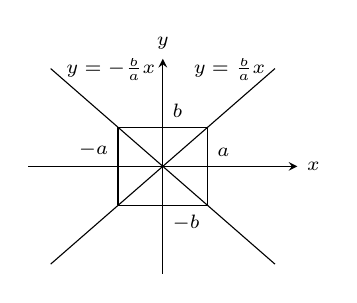
\begin{tikzpicture}[font=\scriptsize,declare function={f(\x)=sqrt(5)/2*sqrt(\x^2-4);fda(\x)=sqrt(5)/2*\x;fdb(\x)=-sqrt(5)/2*\x;}]
\pgfmathsetmacro{\b}{sqrt(5)}
\pgfmathsetmacro{\a}{2}
\pgfmathsetmacro{\n}{\b/2*sqrt(3.5*3.5-4)}
\begin{axis}[width=5cm,axis lines=middle,xlabel={$x$},ylabel={$y$},xlabel style={at={(current axis.right of origin)},anchor=west},ylabel style={at={(current axis.above origin)},anchor=south},xtick={\empty},ytick={\empty},enlargelimits=true, xmin=-5, xmax=5, ymin=-5.123,ymax=5.123]
\addplot[]plot coordinates {(-\a,-\b)(-\a,\b)(\a,\b)(\a,-\b)(-\a,-\b)};
\addplot[]plot coordinates{(-\a,0)}node[above left]{$-a$};
\addplot[]plot coordinates{(\a,0)}node[above right]{$a$};
\addplot[]plot coordinates{(0,\b)}node[above right]{$b$}  {(0,-\b)}node[below right]{$-b$};
\addplot[domain=-5:5]{fda(x)}node[left]{$y=\frac{b}{a}x$};
\addplot[domain=-5:5]{fdb(x)}node[pos=0,right,xshift=0.5ex]{$y=-\frac{b}{a}x$};
\end{axis}
\end{tikzpicture}
\caption{}
\end{subfigure}\hfill
\begin{subfigure}{0.3\textwidth}
\centering
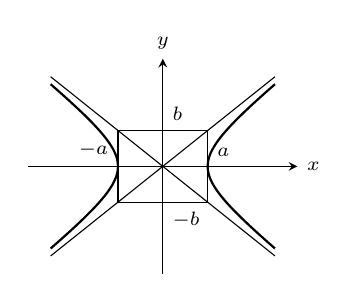
\begin{tikzpicture}[font=\scriptsize,declare function={f(\x)=sqrt(5)/2*sqrt(\x^2-4);fda(\x)=sqrt(5)/2*\x;fdb(\x)=-sqrt(5)/2*\x;}]
\pgfmathsetmacro{\a}{2}
\pgfmathsetmacro{\c}{3}
\pgfmathsetmacro{\b}{sqrt(\c^2-\a^2)}
\pgfmathsetmacro{\n}{\b/2*sqrt(3.5*3.5-4)}
\begin{axis}[width=5cm,axis lines=middle,xlabel={$x$},ylabel={$y$},xlabel style={at={(current axis.right of origin)},anchor=west},ylabel style={at={(current axis.above origin)},anchor=south},xtick={\empty},ytick={\empty},enlargelimits=true]
\addplot[]plot coordinates {(-\a,-\b)(-\a,\b)(\a,\b)(\a,-\b)(-\a,-\b)};
\addplot[]plot coordinates{(-\a,0)}node[above left]{$-a$};
\addplot[]plot coordinates{(\a,0)}node[above right]{$a$};
\addplot[]plot coordinates{(0,\b)}node[above right]{$b$}  {(0,-\b)}node[below right]{$-b$};
\addplot[domain=-5:5]{fda(x)};
\addplot[domain=-5:5]{fdb(x)};
\addplot[thick,domain=2:2.25]{f(x)};
\addplot[thick,domain=2.25:5]{f(x)};
\addplot[thick,domain=2:2.25]{-f(x)};
\addplot[thick,domain=2.25:5]{-f(x)};
\addplot[thick,domain=2:2.25](-x,{f(x)});
\addplot[thick,domain=2.25:5](-x,{f(x)});
\addplot[thick,domain=2:2.25](-x,{-f(x)});
\addplot[thick,domain=2.25:5](-x,{-f(x)});
\end{axis}
\end{tikzpicture}
\caption{}
\end{subfigure}
\caption{متقارب کی مدد سے قطع زائد کی ترسیم۔}
\label{شکل_مخروط_متقارب_سے_قطع_زائد}
\end{figure}

\ابتدا{مثال}\شناخت{مثال_مخروط_ماسکہ_افقی_محور_پر}\ترچھا{محور \عددی{x} پر ماسکے}\\
درج ذیل قطع زائد کی مساوات ہے (شکل \حوالہ{شکل_مثال_مخروط_ماسکہ_افقی_محور_پر})
\begin{align*}
\frac{x^2}{4}-\frac{y^2}{5}=1
\end{align*}
جس میں \عددی{a^2=4} اور \عددی{b^2=5} ہیں (مساوات \حوالہ{مساوات_مخروط_قطع_زائد})۔ یوں درج ذیل ہوں گے۔
\begin{align*}
c&=\sqrt{a^2+b^2}=\sqrt{4+5}=3&&\text{\RL{مرکز سے ماسکہ تک فاصلہ}}\\
(\pm c,0)&=(\pm 3,0)&&\text{ماسکے}\\
(\pm a,0)&=(\pm 2,0)&&\text{راس}\\
y&=\pm \frac{\sqrt{5}}{2}x&&\text{متقارب}
\end{align*}
\انتہا{مثال}
%================
\begin{figure}
\centering
\begin{minipage}{0.45\textwidth}
\centering
\begin{tikzpicture}[declare function={f(\x)=sqrt(5)/2*sqrt(\x^2-4);fd(\x)=sqrt(5/4)*\x;}]
\begin{axis}[clip=false,small,axis lines=middle,xlabel={$x$},ylabel={$y$},xlabel style={at={(current axis.right of origin)},anchor=west}, ylabel style={at={(current axis.above origin)},anchor=south},xtick={\empty},ytick={\empty}]
\addplot[domain=2:2.5]{f(x)};
\addplot[domain=2.5:8]{f(x)};
\addplot[domain=2:2.5]{-f(x)};
\addplot[domain=2.5:8]{-f(x)};
\addplot[domain=2:2.5](-x,{f(x)});
\addplot[domain=2.5:8](-x,{f(x)});
\addplot[domain=2:2.5](-x,{-f(x)});
\addplot[domain=2.5:8](-x,{-f(x)});
\addplot[domain=-8:8]{fd(x)}node[left,yshift=1ex]{$y=\frac{\sqrt{5}}{2}x$};
\addplot[domain=-8:8]{-fd(x)}node[pos=0,right,yshift=1ex]{$y=-\frac{\sqrt{5}}{2}x$};
\addplot[]plot coordinates {(3,0)}node[circ]{}node[above right]{$F(3,0)$}   {(-3,0)}node[circ]{}node[above left]{$F(-3,0)$};
\addplot[]plot coordinates {(2,0)}node[circ]{}node[pin=-40:{$2$}]{}  {(-2,0)}node[circ]{}node[pin=-140:{$-2$}]{};
\addplot[]plot coordinates {(4,4)}node[right,font=\scriptsize]{$\frac{x^2}{4}-\frac{y^2}{5}=1$};
\end{axis}
\end{tikzpicture}
\caption{قطع زائد (مثال \حوالہ{مثال_مخروط_ماسکہ_افقی_محور_پر})}
\label{شکل_مثال_مخروط_ماسکہ_افقی_محور_پر}
\end{minipage}\hfill
\begin{minipage}{0.45\textwidth}
\centering
\begin{tikzpicture}[declare function={f(\x)=2/sqrt(5)*sqrt(\x^2+5);fd(\x)=sqrt(4/5)*\x;}]
\begin{axis}[clip=false,small,axis lines=middle,xlabel={$x$},ylabel={$y$},xlabel style={at={(current axis.right of origin)},anchor=west}, ylabel style={at={(current axis.above origin)},anchor=south},xtick={\empty},ytick={\empty}]
\addplot[domain=-6:6]{f(x)};
\addplot[domain=-6:6]{-f(x)};
\addplot[domain=-6:6]{fd(x)}node[pos=0.75,right,yshift=-0.5ex]{$y=\frac{2}{\sqrt{5}}x$};
\addplot[domain=-6:6]{-fd(x)}node[pos=0.25,left,yshift=-0.5ex]{$y=-\frac{2}{\sqrt{5}}x$};
\addplot[]plot coordinates {(0,3)}node[circ]{}node[above right]{$F(0,3)$}   {(0,-3)}node[circ]{}node[below right]{$F(0,-3)$};
\addplot[]plot coordinates {(0,2)}node[circ]{}node[below left]{$2$}  {(0,-2)}node[circ]{}node[above left]{$-2$};
\addplot[]plot coordinates {(1,5)}node[above right]{$\frac{y^2}{4}-\frac{x^2}{5}=1$};
\end{axis}
\end{tikzpicture}
\caption{قطع زائد (مثال \حوالہ{مثال_مخروط_ماسکہ_عمودی_محور_پر})}
\label{شکل_مثال_مخروط_ماسکہ_عمودی_محور_پر}
\end{minipage}
\end{figure}

\ابتدا{مثال}\شناخت{مثال_مخروط_ماسکہ_عمودی_محور_پر}
درج ذیل قطع زائد کو  مثال \حوالہ{مثال_مخروط_ماسکہ_افقی_محور_پر} کے قطع زائد میں \عددی{x} اور \عددی{y} کو ایک دوسرے کے ساتھ بدل کر حاصل کیا گیا ہے۔ 
\begin{align*}
\frac{y^2}{4}-\frac{x^2}{5}=1
\end{align*}
اس قطع زائد کے راس عمودی محور پر پائے جائیں گے (شکل \حوالہ{شکل_مثال_مخروط_ماسکہ_عمودی_محور_پر})۔ اب بھی \عددی{a^2=4} اور \عددی{b^2=5} ہوں گے۔یوں درج ذیل ہو گا۔
\begin{align*}
c&=\sqrt{a^2+b^2}=\sqrt{4+5}=3&&\text{\RL{مرکز سے ماسکہ تک فاصلہ}}\\
(0,\pm c)&=(0,\pm 3)&&\text{ماسکے}\\
(0,\pm a)&=(0,\pm 2)&&\text{راس}\\
&(0,0)&&\text{مرکز}\\
y&=\pm \frac{2}{\sqrt{5}}x&&\text{متقارب}
\end{align*}
\انتہا{مثال}
%==================

\جزوحصہء{عکسی خواص}
قطع مکافی کا اہم ترین استعمال بطور  شعاع اور ریڈیو امواج کا عاکس ہے۔ قطع مکافی کے ماسکہ سے خارج شعاع، قطع مکافی کے محور کے متوازی منعکس ہوتا ہے۔ یہ خاصیت ہاتھ بتی اور گاڑیوں کی اگلی بتیوں میں بروئے کار لایا جاتا ہے۔ اس کے علاوہ خرد امواج نشر کرنے کے لئے بھی قطع مکافی اینٹینا استعمال کیا جاتا ہے جو نقطہ منبع سے خارج برقناطیسی امواج کو ایک محدود شعاع  کی صورت میں خارج کرتا ہے۔ اس کے برعکس قطع مکافی عاکس کے محور کے متوازی آمد  برقناطیسی امواج عاکس کے ماسکہ پر مرکوز کیے جاتے ہیں۔اس خاصیت کی بنا ٹیلی وژن کا ڈش اینٹینا یا ریڈیو دوربین  کمزور اشارات کو اکٹھے کر کے زیادہ طاقتور اشارہ حاصل کرتا ہے۔
اسی طرح سورج کی روشنی کو ایک نقطہ پر مرتکز کیا جا سکتا ہے۔

ایک ترخیم کو اس کے محور کے گرد گھما کر سطح طواف پیدا کیا جا سکتا ہے جو \اصطلاح{ترخیمی سطح}\فرہنگ{ترخیمی سطح}\حاشیہب{ellipsoid}\فرہنگ{ellipsoid} کہلاتا ہے۔اس کی اندرونی سطح پر چاندی کی تہہ لگا کر آئینہ بنایا جا سکتا ہے۔ ایک ماسکہ سے خارج شعاع دوسرے ماسکہ پر منعکس ہو گا۔ ترخیمی سطح اسی طرح آواز کو بھی ایک ماسکہ سے دوسرے ماسکہ منتقل کرتا ہے۔ اس خاصیت کو استعمال کرتے ہوئے کمرہ سرگوشی بنایا جا سکتا ہے جس میں ایک ماسکہ پر بیٹھا شخص دوسرے ماسکہ پر بیٹھے شخص کے ساتھ سرگوشی سے باتیں کر سکتا ہے۔ کمرہ سرگوشی میں موجود باقی لوگ ان کی باتیں سننے  سے قاصر ہوں  گے۔ ہوائی جہازوں کی کارکردگی پر ہوائی سرنگ میں غور کیا جاتا ہے۔ جہاز کے شور پر غور کرتے ہوئے نقطہ غور کو ترخیمی سطح کے ایک ماسکہ پر رکھا جاتا ہے جبکہ مائکروفون  کو  اس کی دوسرے ماسکہ پر رکھا جاتا ہے۔ دیگر نقطوں سے پیدا شور کے اثر کو یوں بہت کم کرنا ممکن ہوتا ہے۔

قطع زائد آئینہ کے ایک ماسکہ پر آمد شعاع کو آئینہ دوسرے ماسکہ پر بھیجتا ہے۔ قطع مکافی سطح، ترخیمی سطح اور قطع مکافی سطحوں کے خواص کو استعمال کرتے ہوئے جدید دور بین تیار کیے جاتے ہیں۔   


